\documentclass{article}
\usepackage[utf8]{inputenc}
\usepackage[margin = 0.8in]{geometry}
\usepackage{graphicx}
\usepackage{amsmath, amssymb}
\usepackage{subcaption}
\usepackage{multirow}
\usepackage{mathtools}
\usepackage{float}
\usepackage{pythonhighlight}


\title{RBE549 - Final Exam}
\author{Keith Chester}
\date{Due date: December 12, 2022}

\begin{document}

\maketitle

\section*{Problem 1}

In this problem, we are tasked with solving an iterative optical flow problem. To compute optical flow, we learned an interative method to update $u(x,y)$, $v(x,y)$ at each iteration, according to:

\begin{equation}
    \begin{bmatrix}
        u(x,y) \\ v(x,y)
    \end{bmatrix}^2 = \begin{bmatrix}
        \lambda I_x ^2 + 4 && \lambda I_x I_y \\
        \lambda I_x I_y && \lambda I_y^2 + 4
    \end{bmatrix}^{-1}
    \begin{bmatrix}
        \sum_{n\epsilon \textit{neighbors}(x,y)} u^{old}(n)-\lambda I_x I_t \\
        \sum_{n\epsilon \textit{neighbors}(x,y)} v^{old}(n)-\lambda I_y I_t \\
    \end{bmatrix}
\end{equation}

We are asked to consider a local coordinate frame $(x',y')$ where $x'$ is aligned with the image gradient and $y'$ is perpendicular to the image gradient. Likewise, $(u',v')=(\frac{dx'}{dt}, \frac{dy'}{dt})$ are the image velocities in this frame. In this coordinate frame,

\begin{equation}
    I_{x'} = \sqrt{I_x^2 + I_y^2}\textit{ and } I_{y'} = 0
\end{equation}

We wish to show that the update equations:

\begin{equation}
    \begin{bmatrix}
        u'(x,y) \\ v'(x,y)
    \end{bmatrix}^2 = \begin{bmatrix}
        \lambda I_{x'}^2 + 4 && \lambda I_{x'} I_{y'} \\
        \lambda I_{x'} I_{y'} && \lambda I_{y'}^2 + 4
    \end{bmatrix}^{-1}
    \begin{bmatrix}
        \sum_{n\epsilon \textit{neighbors}(x,y)} u'^{old}(n)-\lambda I_{x'} I_t \\
        \sum_{n\epsilon \textit{neighbors}(x,y)} v'^{old}(n)-\lambda I_{y'} I_t \\
    \end{bmatrix}
\end{equation}

\noindent ...can reduce to

\begin{equation}
    u'^{new}(x,y)=\bar{u}'^{old}- \frac{I_{x'}^2\bar{u}'^{old} + I_{x'}I_t}{I_{x'}^2+\frac{4}{\lambda}}
\end{equation}

\begin{equation}
    v'^{new}(x,y)=\bar{v}'^{old}
\end{equation}

\noindent. To do this, we first expand our second term to an equivalnet form to make matters easier for us to work with. Specifically, the inverse of a $2x2$ matrix is:

\begin{equation}
    \begin{bmatrix}
        a & b \\
        c & d
    \end{bmatrix}^{-1} =
    \frac{1}{ad-bc}
    \begin{bmatrix}
        d & -b \\
        -c & a
    \end{bmatrix}
\end{equation}

\noindent ...and thus...

\begin{equation}
    \begin{bmatrix}
        \lambda I_x^2 + 4 & \lambda I_x I_y \\
        \lambda I_x I_y & \lambda I_y^2 + 4
    \end{bmatrix}^{-1} =
    \frac{1}{(\lambda I_x^2 + 4)(\lambda I_y^2 + 4)- \lambda I_x I_y \lambda I_x I_y}
    \begin{bmatrix}
        \lambda I_y^2 + 4 & -\lambda I_x I_y \\
        -\lambda I_x I_y & \lambda I_y^2 + 4
    \end{bmatrix}
\end{equation}

\noindent ...which simplifies to:

\begin{equation}
    \frac{1}{4 \lambda I_x^2 + 4\lambda I_y^2 + 16}
    \begin{bmatrix}
        \lambda I_y^2 + 4 & -\lambda I_x I_y \\
        -\lambda I_x I_y & \lambda I_x^2 + 4
    \end{bmatrix}
\end{equation}

\noindent From here we'll look $\bar{u}'^{new}$.


\section*{Problem 2}

We can represent an object by its boundary, $(x(s),y(s)),0\leq s \leq S$, where $S$ is the length of the object's boundary and $s$ is distance along that boundary from some arbitrary starting point. Combine $x$ and $y$ into a single complex funcion $z(s)=x(s)+jy(s)$. The Discrete Fourier Transform (DFT) of $z$ is:

\begin{equation}
    Z(k) = \sum^{S-1}_{s=0} e^{-2\pi j \frac{ks}{S}} z(s), 0\leq k \leq S-1
\end{equation}

We can use the coefficients $Z(k)$ to represent the object boundary. The limit on $s$ is $S-1$ because for a closed contour $z(S)=z(0)$. The Inverse Discrete Fourier Transform is:

\begin{equation}
    z(s) = \frac{1}{S} \sum_{k=0}^{S-1} e^{+2\pi j \frac{ks}{S}} Z(k), 0 \leq s \leq S-1
\end{equation}

\subsection*{A}

Suppose that the object is translated by $(\Delta x, \Delta y)$, that is, $z'(s)=z(s) + \Delta x + j \Delta y$. How is $z'$'s DFT $Z'(k)$ related to $Z(k)$?


\begin{equation}
    Z(k) = \sum^{S-1}_{s=0} e^{-2*\pi j \frac{ks}{S}} z(s), 0\leq k \leq S-1
\end{equation}

\noindent Which we can define $z'(s)$ as:

\begin{equation}
    z'(s) = z(s) + \Delta x + j \Delta y
\end{equation}

\noindent If we plug this into our original equation, we get...

\begin{equation}
    Z'(k) = \sum_{s=0}^{S-1} e^{-2\pi j \frac{ks}{S}}z(s) + \sum_{s=0}^{S-1} e^{-2\pi j \frac{ks}{S}} (\Delta x + j \Delta y) (1)
\end{equation}

\noindent Here we see that we have a segment that is equivalent to oru defined $Z(k)$, so we can simplify by expressing:

\begin{equation}
    Z(k) + (1) (\Delta x + j \Delta y) \sum_{s=0}^{S-1} e^{-2\pi j \frac{ks}{S}}
\end{equation}

\noindent With $\Delta x$ and $j \Delta y$ isolated, we can use a table of known Fourier Transforms to identify the resulting conversion. Based on our problem's definition $\Delta X$ and $\Delta y$ are both constants, so we can state that:

\begin{equation}
    Z'(k) = Z(k) + (\Delta x + j \Delta y) \sigma(\frac{2 \pi k}{S})
\end{equation}

\noindent ...where $\frac{1}{S}$ acts as our scaling factor.

\subsection*{B}

In this section, we are asked to suppose that the object is scaled by an integer constant $c$, that is $z'(s)=cz(s)$. For simplicity, we are to assume that $S'=S$. How is $Z'(k)$ as the DFT of $z'$ related to $Z(k)$?

\noindent Starting with our definition of $Z(k)$, which is our Fourier Transform of $z(s)$ as defined earlier:

\begin{equation}
    Z(k) = \sum^{S-1}_{s=0} e^{-2\pi j \frac{ks}{S}} z(s), 0\leq k \leq S-1
\end{equation}

\noindent If we then define $z'(s)$ as above, $z'(s)=cz(s)$, we can plug it into our Fourier Transform:

\begin{equation}
    Z'(k) = \sum^{S-1}_{s=0} e^{-2\pi j \frac{ks}{S}} cz(s)
\end{equation}

\noindent Since $c$ is a constant, we know we can pull it in front of the fourier Transform like so:

\begin{equation}
    Z'(k) = c \sum^{S-1}_{s=0} e^{-2\pi j \frac{ks}{S}} z(s) 
\end{equation}

\noindent ...and further simplified:

\begin{equation}
    Z'(k) = c Z(k)
\end{equation}

\noindent ...which shows that multiplying our time series function by a given scalar simply multipies our frequncy domain by the same scalar.


\subsection*{C}

We wish to know what object has $z(s)=\begin{bmatrix}x_0 + R\cos(\frac{2\pi s}{s})\end{bmatrix}+j\begin{bmatrix}y_0 + R \sin(\frac{2\pi s}{s})\end{bmatrix}$. Below we created a graph drawing the resulting shape, and include the code utilized to generate it. Arbitrary values were chosen for $S$, $r$, $x_0$, and $y_0$ for the sake of plotting.

\begin{figure}[H]
    \centering
    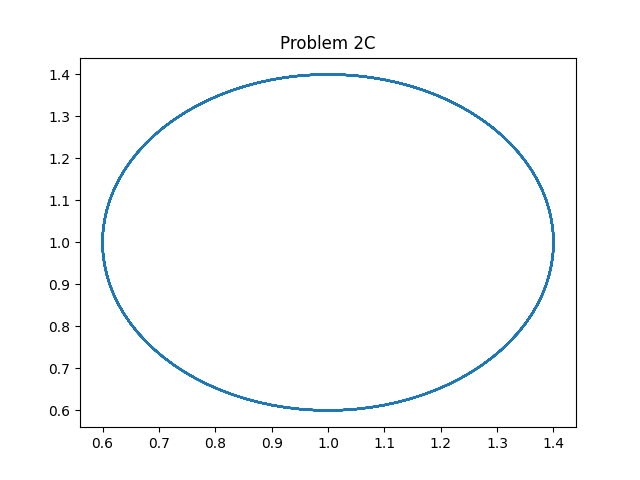
\includegraphics[width = 0.65\textwidth]{imgs/prob2_c.png}
    \caption{Our resulting shape}
    \label{fig:prob2-c}
\end{figure}

\begin{python}
    import numpy as np
    from numpy import cos, sin, pi
    import matplotlib.pyplot as plt
    
    figure = plt.figure()
    plt.title("Problem 2C")
    
    S = 10
    r = 4
    x0 = 1
    y0 = 1
    
    theta = [theta for theta in np.arange(0, S, 0.01)]
    X = [
            x0 + r * cos(2*pi*theta)/S
            for theta in theta
        ]
    Y = [
            y0 + r * sin(2*pi*theta)/S
            for theta in theta
        ]
    
    # Plot the results
    plt.plot(X, Y)
    plt.savefig("./imgs/prob2_c.png")
\end{python}

\subsection*{D}

What is $Z(k)$ corresponding to $z(s)$ from Part C? To do this, we begin wtih our $z(s)$:

\begin{equation}
    z(s)=\begin{bmatrix}x_0 + R\cos(\frac{2\pi s}{s})\end{bmatrix}+j\begin{bmatrix}y_0 + R \sin(\frac{2\pi s}{s})\end{bmatrix}
\end{equation}

We can utilize the inverse of Euler's formula; $\cos(x)=\frac{e^{ix}+e^{-ix}}{2}$ and $\sin(t) = \frac{e^{ix}-e^{-ix}}{2x}$. This allows us to expand our starting equation:

\begin{equation}
    z(s)= x_0 + R\frac{e^{j\frac{2\pi s}{S}} + e^{-j\frac{2\pi s}{S}}}{2} + jy_0 + R\frac{e^{j\frac{2\pi s}{S}}-e^{-j\frac{2\pi s}{S}}}{2}
\end{equation}

\begin{equation}
    z(s) = x_0 + jy_0 + \frac{R}{2} \bigl(e^{j\frac{2\pi s}{S}} + e^{-j\frac{2\pi s}{S}} + e^{j\frac{2\pi s}{S}} - e^{-j\frac{2\pi s}{S}}\bigr)
\end{equation}

\begin{equation}
    z(s)= x_0 + jy_0 + \frac{R}{2} \bigl( 2e^{j\frac{2\pi s}{S}} \bigr)
\end{equation}

\begin{equation}
    z(s)= x_0 + jy_0 + Re^{j\frac{2\pi s}{S}}
\end{equation}

\noindent The Discrete Fourier Transform (DFT) from earlier in our problem we can begin to expand this equation now. Starting with:

\begin{equation}
    Z(k) = \sum^{S-1}_{s=0} e^{-2\pi j \frac{ks}{S}} z(s), 0\leq k \leq S-1
\end{equation}

\noindent ...which can lead us to:

\begin{equation}
    Z(k) = \sum^{S-1}_{s=0} e^{-2\pi j \frac{ks}{S}} \bigl( x_0 + jy_0 + Re^{j\frac{2\pi s}{S}} \bigr)
\end{equation}

\noindent ...constants can be pulled out, leaving us with:

\begin{equation}
    Z(k) = \sum^{S-1}_{s=0} e^{-2\pi j \frac{ks}{S}} (x_0 + jy_0) + R\sum^{S-1}_{s=0} e^{-2\pi j \frac{ks}{S}} e^{j\frac{2\pi s}{S}}
\end{equation}

\begin{equation}
    Z(k) = (x_0 + jy_0) \sum^{S-1}_{s=0} e^{-2\pi j \frac{ks}{S}}  + R\sum^{S-1}_{s=0} e^{-j 2 \pi (k-1)} S
\end{equation}

\noindent We know from a Fourier Transform lookup table we can then convert this to:

\begin{equation}
    Z(k) = (x_0+jy_0)\sigma(\frac{2\pi k}{S}) + \sigma(2\pi \frac{k-1}{S})
\end{equation}



\end{document}